% !TEX root = hazel-LIVE2018.tex

%% \subsection{Live Programming with Type Errors}

\subsection{Example 2: Live Programming with Static Type Errors}
\label{sec:static-errors}


% \begin{subfigure}[t]{\textwidth}
\begin{figure}
\centering
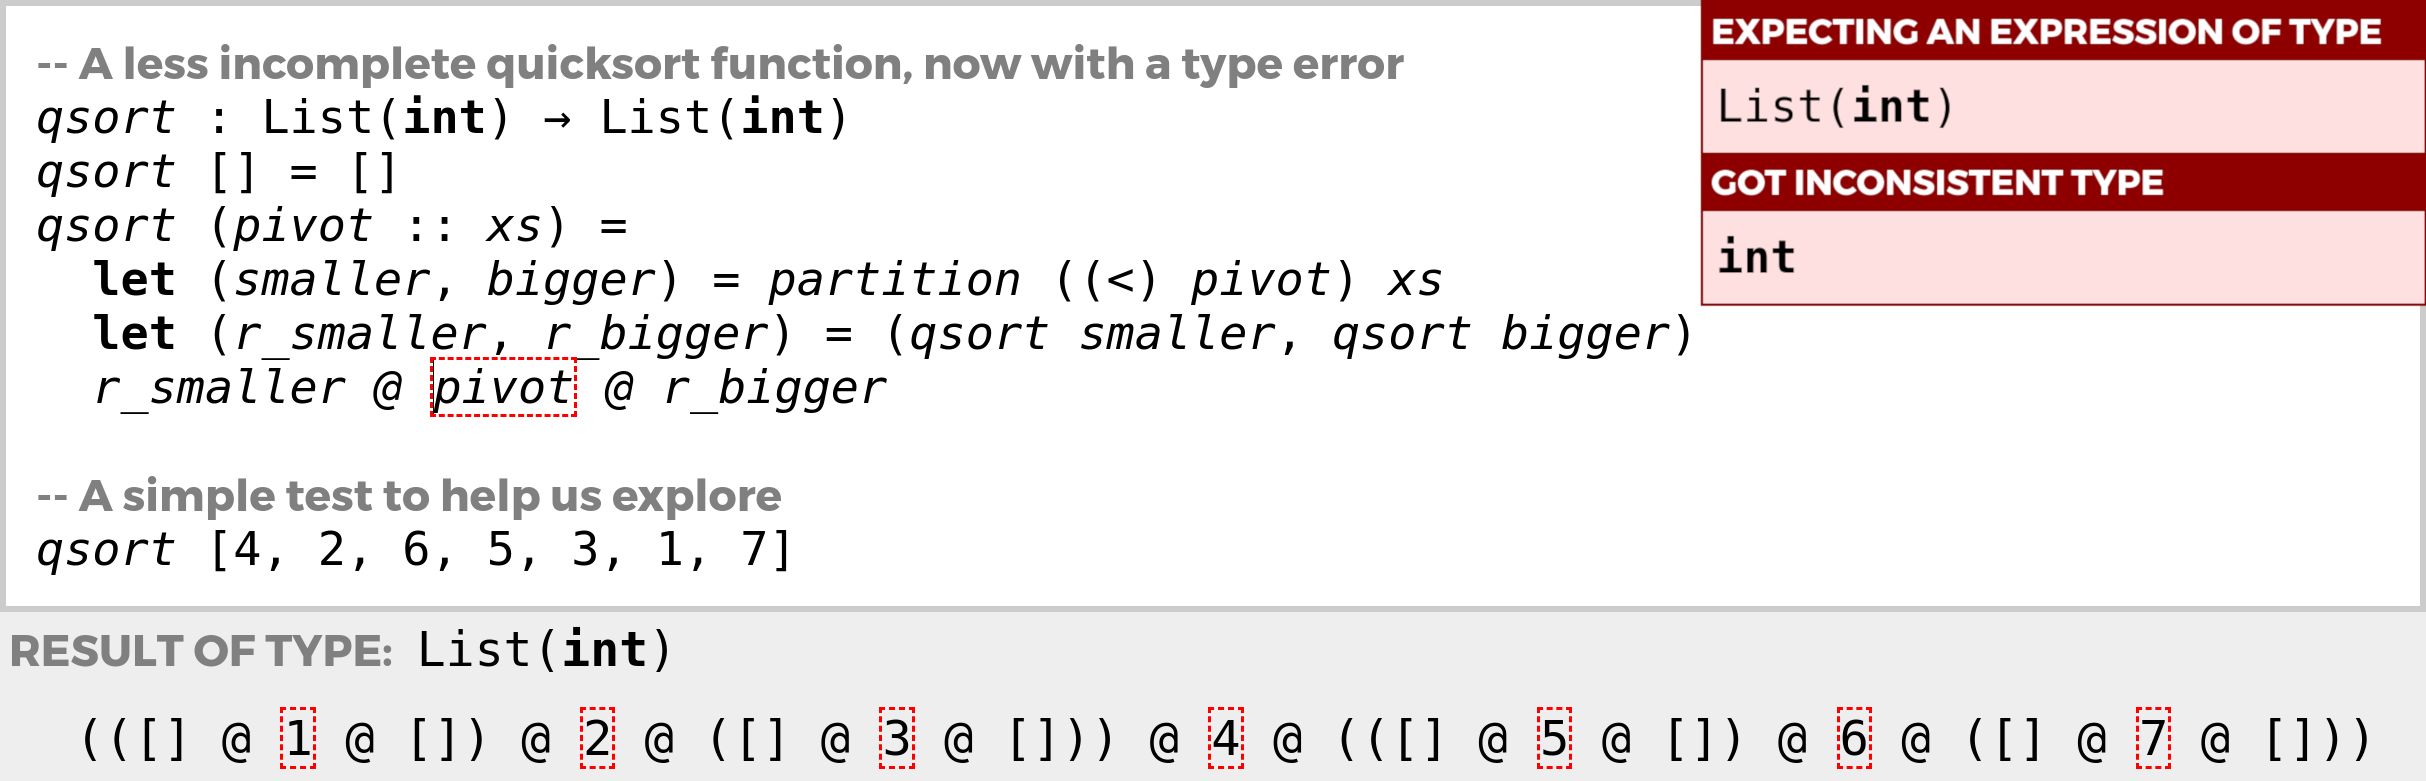
\includegraphics[width=\textwidth,interpolate=false,valign=t]{images/qsort-type-error-inset.png}
% 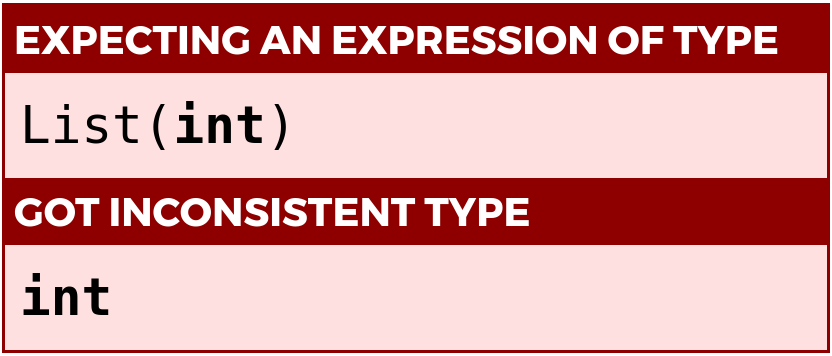
\includegraphics[width=0.28\textwidth,interpolate=false,valign=t]{images/type-inconsistency.png}
\vspace{2px}
\caption{Example 2: Ill-Typed Quicksort}
\label{fig:qsort-type-error}
\vspace{-4px}
\end{figure}
% \end{subfigure}


The previous example was incomplete 
because of \emph{missing} expressions.
%
Now, we discuss programs that are incomplete, 
and therefore conventionally meaningless, because of
\emph{type inconsistencies}. 
%
Let us 
assume that the programmer has filled in hole \li{1} in the previous example 
as shown in Fig.~\ref{fig:qsort-type-error}. 
Because the result computed in the previous example recorded the environment around every
instance of hole \li{1} in the result, a  new result can be computed from the previous result by performing 
contextual substitution (a concept from contextual modal type theory \cite{Nanevski2008})  and resuming evaluation, rather than restarting evaluation entirely.
In larger examples, this could significantly impact evaluation time, which is  
important to perceived liveness \cite{DBLP:conf/icse/Tanimoto13}. 

The programmer appears to be on the right track conceptually
in recognizing that the pivot needs to appear between the 
smaller and bigger elements. 
However, the types do not quite work out: the \li{@} operator here
performs list concatenation, but the pivot is an integer. 
Most compilers and editors will report a static error message
to the programmer in this case, and \Hazel 
follows suit in the type inspector (shown inset in Fig.~\ref{fig:qsort-type-error}). 
However, our argument is that the presence of a static type error should not cause all feedback about 
the dynamic behavior of the program to ``flicker out'' or ``go stale'' --
after all, there are perfectly meaningful parts of the program (both nearby
and far away from the error) 
whose dynamic behavior may be of interest. Evaluation can also assist the programmer in understanding the type error by presenting concrete values \cite{Seidel2016}.
% After all,
% the error is localized and there is perfectly good code elsewhere 
% in the program (if not nearby, then perhaps far away).

Our approach, following the prior work of \citet{popl-paper}, 
is to semantically internalize the ``red outline'' around
type inconsistencies, representing it as a \emph{non-empty hole}.
Evaluation safely proceeds past a non-empty hole just as if it were an empty hole.
The semantics also associates an environment with each instance of a non-empty hole,
so we can use the live context inspector essentially as in Fig.~\ref{fig:qsort-sidebars} (not shown). 
Evaluation proceeds inside the hole, so that 
feedback about the type-inconsistent expression, which might ``almost'' be correct, is available. 
In this case, the result at the bottom of Fig.~\ref{fig:qsort-type-error}
reveals that the programmer is on the right track: the list elements 
appear in the correct order.
They simply have not been combined correctly.



% For example, consider the following two definitions.

% \begin{lstlisting}
% let bad_bool : bool = ?? 0 ??_bad_bool;

% let bad_int : int = 1 + ?? true ??_bad_int_second_argument;
% \end{lstlisting}

% \noindent
% %
% These two definitions are ill-typed under standard typing disciplines.
% %
% In contrast, \citet{popl-paper} present a bidirectional type system that assigns
% types to both, by wrapping type-inconsistent expressions (\li{0} on line
% \rkc{XXX} and \li{true} on line \rkc{XXX} above) in \emph{non-empty} holes.
% %
% Non-empty holes prevent local type inconsistencies from polluting the rest of
% the program surrounding it, which may or may not itself contain additional
% inconsistencies.

\begin{comment}
\overviewExample{2}{Sum List}
%
Consider the following buggy program (observed during an undergraduate
functional programming course~\cite{Seidel2016}) that attempts to sum a list
integers.
%
The error is that the base case produces a list rather than an integer.

\begin{lstlisting}
sum_list : list(int) -> int
sum_list [] = ?[]?
sum_list (n:ns) = n + sum_list ns
\end{lstlisting}

\noindent
%
Because the list expression on line 2 does not have type \li{int} as required,
it is wrapped in a (non-empty) hole by the bidirectional type
checker~\cite{popl-paper}.
%
Rather than trying to debug the error based on the static error, the programmer
may wish to trying running the function anyway by calling, say, \li{sum_list(2)}.
%
\HazelnutLive{} runs and produces the indeterminate expression \li{3 + ?[]?}.
%
By observing that the hole expression is being added to the integer \li{3}, he
realizes that it needs to be an integer, specifically, \li{0}.
%
Compared to the trace displayed by \citet{Seidel2016}, the indeterminate result
produced by \HazelnutLive{} is ``flattened'' because the expression \li{1 + 2}
successfully proceeded to evaluate despite the error elsewhere.
\end{comment}

%% TODO fold error from Erwig paper.
%% %
%% see that final call on stack does have the right answer, but
%% it's wrapped in a singleton list when the expected type is not
%% a list.
%% %
%% fix is to remove the list, the rest of the computation remains
%% the same, but b/c they were all wrapped in holes, need to re-run.
%% %
%% (add some mechanism for type-consistent non-empty-holes...)

\begin{comment}

\overviewExample{4}{Stutter}
%
Consider the following function which attempts to produce a
list where every element is repeated twice (borrowed from \citet{Osera2015}).
%
The combiner function to \li{List.foldr} needs to produce a \li{list(int)}, but
it produces a \li{list(list(int)} instead.

\begin{lstlisting}
stutter : list(int) -> list(int)
stutter xs = List.foldr (\x acc -> ?[x,x]? : acc) [] xs
\end{lstlisting}

\noindent
%
The bidirectional type checker of \citet{popl-paper} wraps the expression
\li{[x,x]} inside a non-empty hole.
%
%% The editor has a choice about which expression to ``blame'' for the error; the
%% entire application that forms the body of the lambda is analyzed against the
%% return type \li{list(int)}, so that is a reasonable choice for the editor to
%% make; another would be to assume that the arguments \li{[x,x]} and \li{acc} are
%% both as intended and that only the function \li{(:)} is type-consistent.
%% %
%% Although one could imagine a setting in which a user would perform this
%% reasoning, let's assume the simplest approach for marking consistencies that
%% wraps the entire application.
%
Running this on \li{stutter [1,2,3]} produces the indeterminate result

\begin{lstlisting}
?  [1,1] : (? [2,2] : (? [[3:3]] ?) ?) ?,
\end{lstlisting}

\noindent
%
which shows the unfolding of \li{List.foldr}.
%
We refer to nested indeterminate computations like this as \rkc{\emph{hole
environment traces} or \emph{hole environment trees}}.
%
The result of the innermost indeterminate expression is \li{[[3,3]]}.
%
The user realizes that there are too many levels of nesting, so
he replaces the \li{(:)} with \li{(@)}, which addresses the type inconsistency
and, when reevaluated, produces the desired result.

\end{comment}
